\subsection{Stoffschluss \hfill ME}
\begin{itemize}
    \begin{scriptsize}
        \item Kraftübertragung durch \textbf{Molekularkräfte}
        \item \textbf{Adhäsion:} Haftkräfte an Kontaktfläche \underline{verschiedener} Werkstoffe
        \item \textbf{Kohäsion:} Haftkräfte an Kontakfläche \underline{eines} Werkstoffes
        \item \textbf{Nachteil:} nicht lösbare Verbindung $\to$ kann nur durch Zerstörung gelöst werden
        \item \textbf{Beispiele:} Kleben / Löten / Schweissen
    \end{scriptsize}
    \begin{footnotesize}
        \mathbox{
        F \leq F_{\text{scher}} = \tau_{\text{szul}} \cdot A \quad \mid \quad \tau = \text{Schubspn.} = \frac{F}{A}
    }
    \centering $A$ = Scherfläche (rot)
    \begin{center}
        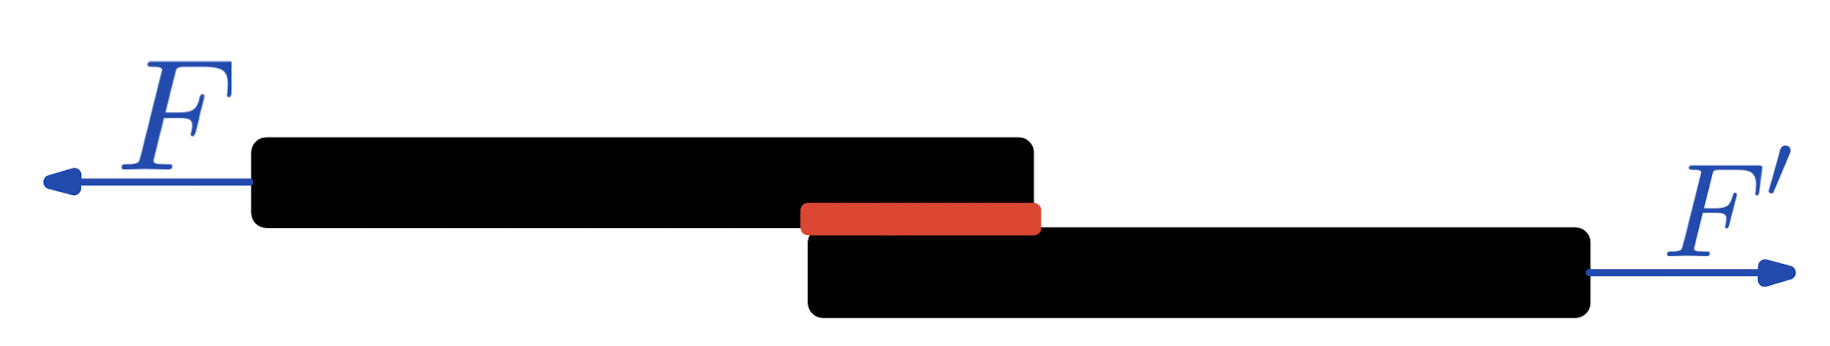
\includegraphics[width = 0.5\linewidth]{src/images/MAEIP_Stoffschluss}
    \end{center}
    \end{footnotesize}
\end{itemize}